\subsection{Designing Output Test} % (fold)
\label{sub:designing_hello_world}

Our first programming task is to extended the classic `Hello World' program to also output some data values, which we will call \textbf{Output Test}. This program will allow you to see all of the different concepts from this chapter in action. A description of the program is shown in Table \ref{tbl:program-creation-hello world description}, and a sample execution is shown in Figure \ref{fig:program-creation-helloworld2}.

\begin{table}[h]
\centering
\begin{tabular}{l|p{12cm}}
  \hline
  \multicolumn{2}{c}{\textbf{Program Description}} \\
  \hline
  \textbf{Name} & \emph{Output Test} \\
  \\
  \textbf{Description} & Displays the text \textbf{`Extended Hello World!'} on the Terminal, followed by \\
                       & \textbf{` 1 + 1 = '} and the result of the calculation 1 + 1, and then \\
                       & \textbf{` Area of a circle with radius 3 = '} and the result of calculating this value. \\
  \hline
\end{tabular}
\caption[Output Test Description]{Description of the \emph{Output Test} program.}
\label{tbl:program-creation-hello world description}
\end{table}

\begin{figure}[h]
   \centering
   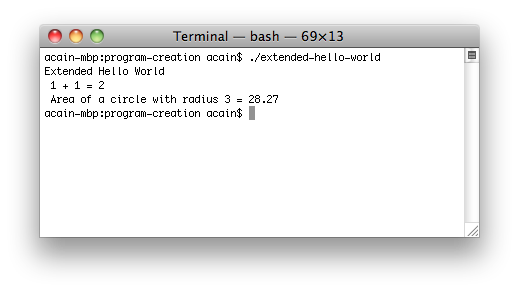
\includegraphics[width=\textwidth]{./topics/program-creation/images/HelloWorld} 
   \caption{Output Test run from the Terminal}
   \label{fig:program-creation-helloworld2}
\end{figure}

To design and implement this program we need to follow a number of steps:

\begin{enumerate}
  \item Understand the problem, and get some ideas on the tasks that need to be performed
  \item Choose the artefacts we will create and use
  \item Map these artefacts to code
  \item Compile and run the program
\end{enumerate}


% \begin{enumerate}
%   \item Determine the programming artefacts that you will need for the program; covered in section \ref{sub:choosing_artefacts_hello_world}. To do this you will need to:
%   \begin{itemize}
%     \item Decide which artefacts to \textbf{create}.
%     \item Select artefacts to \textbf{use} from the Libraries.
%   \end{itemize}
%   \item Determine the sequence of instructions you will need to give the computer for it to use these artefacts to produce the outcome you are looking for.
% \end{enumerate}


% subsection designing_hello_world (end)
\clearpage
\subsection{Understanding Output Test} % (fold)
\label{sub:understanding_output_test}

The first step in creating a program is to analyse the problem, and find related material that we can use to make sure we know what the computer needs to do. You need to understand what the program needs to do before you can start to design the solution.

For this program you need to understand how to calculate the answer of the equation 1 + 1, which is a trivial task, and also how to calculate the area of a circle given its radius. A quick search of the internet and you can find the equation is $PI \times r^2$. Using these equations you have the knowhow needed to calculate the values needed to be output.

% subsection understanding_output_test (end)
\subsection{Choosing Artefacts for Output Test} % (fold)
\label{sub:choosing_artefacts_hello_world}

Designing a program is all about making decisions around how to organise the program's instructions. This means \textbf{deciding} on which artefacts you will \textbf{create}, and which you will \textbf{use}. This chapter has introduced the concept of \textbf{creating} a \nameref{sub:program}, and \textbf{using} \nameref{sub:procedure}s. With these tools it is possible to design simple programs that will get the computer to perform actions by running Procedures in sequence.

The design of \emph{Output Test} requires:

\begin{itemize}
  \item The \textbf{creation} of a \nameref{sub:program}. This Program will contain the instructions to write the three messages to the Terminal.
  \item The \textbf{use} of a procedure to write to the console. Programming languages provide a standard \nameref{sec:program-creation-library} that, amongst other things, contains procedures to write data to the Terminal. This means you can call one of these procedures, passing it the data you want written to the Terminal, and let it take care of the details of how this is done.
\end{itemize}

\bigskip

The design for this program can be documented using a language neutral \textbf{pseudocode}. This isn't code, just a structured textural description of how the program is intended to work. It gives us a way of reasoning about the program we are creating that is independent of the language used to implement it. As this isn't really code it means we can write it without having to worry about the syntax of a specific programming language.

Listing \ref{lst:program-creation-hello-pseudo} shows the pseudocode for the \emph{Output Test} program. This represents the \textbf{Program} that needs to be created, and shows the three \textbf{Procedure Calls} that need to be made. 

\pseudocode{lst:program-creation-hello-pseudo}{Pseudocode for the Output Test program.}{./topics/program-creation/application/HelloWorld.txt}

\csection{In C the procedure to write data to the Terminal is called \texttt{printf}, see \nameref{sub:c_console_output}.}
\passection{Pascal has two procedures to write data to the Terminal, \texttt{Write} and \texttt{WriteLn}. }

% subsection choosing_artefacts (end)
\clearpage
\subsection{Writing the Code for Output Test} % (fold)
\label{sub:writing_the_code_for_output_test}

The pseudocode in Listing \ref{lst:program-creation-hello-pseudo} contains the instructions that will get the computer to perform the actions needed by the \emph{Output Test} program. These instructions are not in a form that can be used by the Computer, which can only use machine code. The next step is therefore to convert these ideas into source code that a compiler can then turn into machine code.

The following two sections, Section \ref{sec:program-creation-in-c} \nameref{sec:program-creation-in-c} and Section \ref{sec:program-creation-in-pas} \nameref{sec:program-creation-in-pas}, contain a description of the syntax needed to create programs in the C and Pascal programming languages. Each section outlines how to write the code so that it can be understood by the compiler. These are expressed as a number of related syntax rules. You will find the rules that you need to create a Program, the rules for calling a Procedure, and the related rules.

The rules themselves are expressed as \textbf{Syntax Diagrams}. An example diagram is shown in Figure \ref{synt:basic-rule}. This diagram shows the syntax related to two rules, \emph{first rule}, and \emph{second rule}, and shows the four main parts of all the Syntax Diagrams.

\begin{enumerate}
  \item Text found at the start of a line, not contained in a box, is the name of a rule. There are two rules in Figure \ref{synt:basic-rule}: \emph{first rule}, and \emph{second rule}.
  \item The arrows show the order in which the parts of the rule are applied. They start at the rule, and point in the direction you need to follow. Each box pointed to by the arrow represents either another rule to apply, or text that must be entered into the code at that point.
  \item The rectangular boxes on the line indicate points where other rules need to be applied. For example, the node  \tikz \node [nonterminal] {second rule}; within the \emph{first rule} indicates that you \textbf{must} apply the \emph{second rule} at this point.
  \item The boxes with rounded corners represent text that must be entered into the code. For example, the node \tikz \node [terminal] {write in the code}; within the \emph{first rule} indicates that you \textbf{must} write the text `\emph{write in the code}' at this point in your code.
\end{enumerate}

\examplesyntax{synt:basic-rule}{An example rule}{basic_rules}

In order to use these Syntax Diagrams, you must know what it is that you want to write in the code. The rules in Figure \ref{synt:basic-rule} indicate that you can write either a \emph{first rule} or a \emph{second rule}. If you want to write a \emph{first rule} you find that rule in the diagram, and then follow it's arrows. Reading the \emph{first rule} indicates that the \emph{second rule} must be applied first. 

The \emph{second rule} tells you that you must write the text `\emph{stuff to}'. The vertical bar at the end of the line indicates the end of the \emph{second rule}. This means at this stage the code is:

\begin{verb}
  stuff to 
\end{verb}

Having finished the \emph{second rule}, you can return back to finish the \emph{first rule}. This indicates that you need to write `\emph{write in the code}' in the code. This is the last part of the \emph{first rule}, and so the code needed to write a \emph{first rule} from the Syntax Diagram in Figure \ref{synt:basic-rule} is shown below.

\begin{verb}
  stuff to write in the code
\end{verb}

For a more realistic example have a look at the Syntax Diagram in Figure \ref{synt:example-identifier}\footnote{ 
The \tikz \node [meta-terminal] {...}; is used as shorthand to avoid having to list all of the characters between `A' to `Z'.}. This shows the rules you need to follow to code an \nameref{sub:identifier}\footnote{Most programming languages have the same rules for identifiers.} in either C or Pascal.

\examplesyntax{synt:example-identifier}{The Syntax Rules for an Identifier}{identifier}

There are three rules in Figure \ref{synt:example-identifier}, the \textbf{identifier} rule itself which uses the rules \textbf{letter} and \textbf{digit}. These rules show arrows that give you \emph{options}, and the ability to \emph{repeat} parts of the rules.

\begin{itemize}
  \item A \textbf{letter} is one alphabetic character: i.e. one of `A' to `Z' or `a' to `z'. This is an example of options in the syntax, where you follow \textbf{one} of the available arrows.
  \item A \textbf{digit} is a single number: i.e. a number between `0' and `9'.
  
  \item The \textbf{identifier} has a more complicated rule, with the following parts:
  \begin{enumerate}
    \item The first thing in an \nameref{sub:identifier} must be either a \emph{letter} or an underscore ( \_ ).
    \item Following this is an example of another kind of option. Here you have the ability to end the rule, allowing you to have identifiers that are a single character, or you can follow the downward arrow to include other letters, digits, and underscores.
    \item Following the downward arrow you have a new option where you can choose to have either a \emph{letter}, a \emph{digit}, or an underscore as the second character in your identifier.
    \item Continuing after this option you have another option where you can return back to repeat the previous step, allowing you to have identifiers with more than one or two characters.
  \end{enumerate}
\end{itemize}

\subsubsection{Using the Syntax Diagrams} % (fold)
\label{ssub:using_the_syntax_diagrams}

The Syntax Diagrams help you to map a Concept to the actual code that needs to be written in your source code. To use these diagrams you must first know what it is that you want to create or use, and then you can look up the related syntax. This is where the pseudocode code comes into play. It contains a description of the things that need to be created. 

Listing \ref{lst:program-creation-hello-pseudo3} shows the pseudocode for the Output Test program. This tells you what needs to be created; you need to create a \nameref{sub:program}. This means you need to find the syntax that tells you the rules of how a \emph{Program} is written in C or Pascal. 

\pseudocode{lst:program-creation-hello-pseudo3}{Pseudocode for the \emph{Output Test} program (repeated from Listing \ref{lst:program-creation-hello-pseudo})}{./topics/program-creation/application/HelloWorld.txt}

The pseudocode also indicates that you need to find the rules related to \nameref{sub:procedure call}s. For this Program you need to code three procedure calls within the Program's instructions. The language's syntax will tell you how you code these instructions, the Syntax for the Program will show you where these instructions are written.

% subsubsection using_the_syntax_diagrams (end)

\subsubsection{How the Syntax is Presented} % (fold)
\label{ssub:how_the_syntax_is_presented}

The C and Pascal Syntax needed to create a program are shown in Section \ref{sec:program-creation-in-c} \nameref{sec:program-creation-in-c} and Section \ref{sec:program-creation-in-pas} \nameref{sec:program-creation-in-pas}. Each part of the Syntax is presented on its own page that shows the Syntax Diagram followed by an example and some notes. The best way to approach this is to do the following:

\begin{enumerate}
  \item Find the page with the Syntax rule you are interested in knowing about.
  \item Have a quick look at the Syntax Diagram and the rules it contains. Read each rule, and get a basic feel for how it is going to come together for your program.
  \item Read the example to see one way of using the Rule. The Syntax Diagram can be used to create any number of variations of the rule, the example gives you at least one way these rules can be coded.
  \item Return to the diagram and make sure you can match each part of the example back to the rule that created it.
  \item Now look up any related rules that are not explained on this rule's page. For example, a \nameref{sub:program} will use the \nameref{sec:program-creation-statement} rule to code its instructions. The actual rule for a Statement will have its own page. When you read the rules for a Program you will need to also find the page with the rules for a Statement so that you know how to code these within the Program.
\end{enumerate}

As you follow this process it is also a good idea to try to use these rules in your own program. Have your code editor open, and see if you can follow the rules or mimic the examples to start building your own program's code. You can also try typing in some of the examples to see how they work.

% subsubsection how_the_syntax_is_presented (end)

% subsection writing_the_code_for_output_test (end)

\subsection{Compiling and Running Output Test} % (fold)
\label{sub:compiling_and_running_output_test}

The previous sections have shown the pseudocode for the \emph{Output Test} program. These steps can be coded using either C or Pascal into a source code file. In order to actually use these instructions you will first need to \textbf{compile} the source code file. This will produce an executable file that you can run.

We are going to start using a \textbf{command line compiler}. You will run this compiler within a text based environment, the \textbf{Terminal}. 

\begin{itemize}
  \item On Ubuntu \textbf{Linux} you can find the Terminal in the \textbf{Accessories} folder within \textbf{Applications}. See Figure \ref{fig:program-creation-ubuntu-terminal}.
  \item On \textbf{MacOS} you can find the Terminal in the \textbf{Utilities} folder within \textbf{Applications}. See Figure \ref{fig:program-creation-macos-terminal}.
  \item On \textbf{Windows} you will need to download and install \emph{MinGW}, making sure to select the \emph{MinSYS} option during the install process. The \emph{MinGW Shell} is then the equivalent of Terminal on the other operating systems. You will find this in \textbf{Program Files}, \textbf{MinGW}. See Figure \ref{fig:program-creation-mingw-shell}.
\end{itemize}

\begin{figure}[p]
   \centering
   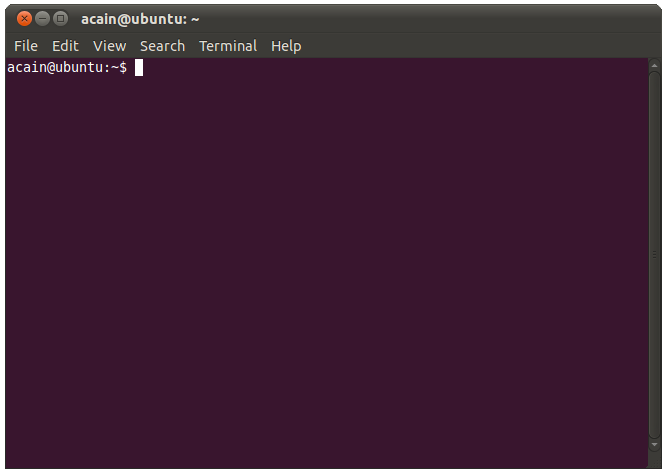
\includegraphics[width=0.6\textwidth]{./topics/program-creation/images/UbuntuTerminal} 
   \caption{Terminal on Ubuntu Linux}
   \label{fig:program-creation-ubuntu-terminal}
\end{figure}

\begin{figure}[p]
   \centering
   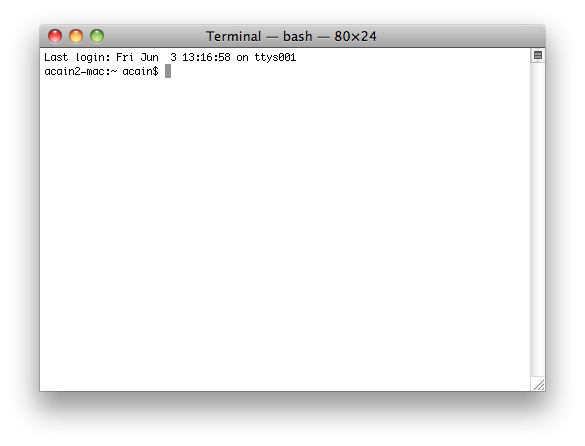
\includegraphics[width=0.6\textwidth]{./topics/program-creation/images/MacOSTerminal} 
   \caption{Terminal on MacOS}
   \label{fig:program-creation-macos-terminal}
\end{figure}

\begin{figure}[p]
   \centering
   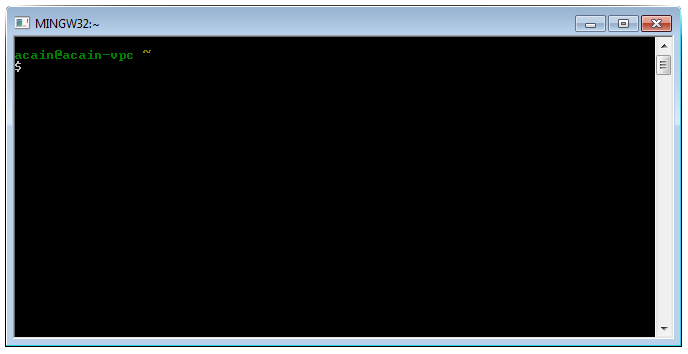
\includegraphics[width=0.6\textwidth]{./topics/program-creation/images/MinGWShell} 
   \caption{MinGW Shell, the Terminal for Windows}
   \label{fig:program-creation-mingw-shell}
\end{figure}

Once you are in the Terminal you have the ability to run a number of text based commands. These commands instruct the computer to perform actions for you.

\begin{itemize}
  \item \textbf{pwd} stands for \emph{Present Working Directory}, and shows you where you are in the file system.
  \item \textbf{ls} stands for \emph{List} and it prints out a list of the files that are in the current directory.
  \item \textbf{cd} stands for \emph{Change Directory} and it moves you to another directory. 
\end{itemize}

To compile your program you need to do the following:

\begin{enumerate}
  \item Change into the directory where your code is located using the \textbf{cd} command. For example, if your code is in a \emph{Code} folder in your \emph{Documents} folder you would use:
  \begin{itemize}
    \item \textbf{Linux}: \texttt{cd /home/username/Documents/Code}
    \item \textbf{MacOS}: \texttt{cd /Users/username/Documents/Code}
    \item \textbf{Windows}: \texttt{cd /c/Users/username/Documents/Code}\footnote{This example moves you into the \texttt{c:{\textbackslash}Users{\textbackslash}username{\textbackslash}Documents{\textbackslash}Code} folder. You need to use the /c/ to refer to the C drive. }
  \end{itemize} 
  \item Run the compiler, passing in the name of the file you want to compile. See the language specific notes below
  \item Execute the program using \texttt{./OutputTest}
\end{enumerate}

\csection{
The C compiler is called \textbf{gcc}. To compile your \emph{Output Test} program you will need to run the following: \bashcode{}{}{code/c/program-creation/compile-output-test.sh}
}

\passection{
The Pascal compiler is called \textbf{fpc}. To compile your \emph{Output Test} program you will need to run the following: \bashcode{}{}{code/pascal/program-creation/compile-output-test.sh}
}

\clearpage
Figure \ref{fig:program-creation-complete-linux-version} shows an example of the instructions needed to compile and run the C version of the \emph{Output Test} program on Linux. Figure \ref{fig:program-creation-complete-linux-version-1} shows an example of the instructions needed to compile and run the Pascal version of the \emph{Output Test} program on Linux.

\begin{figure}[h]
   \centering
   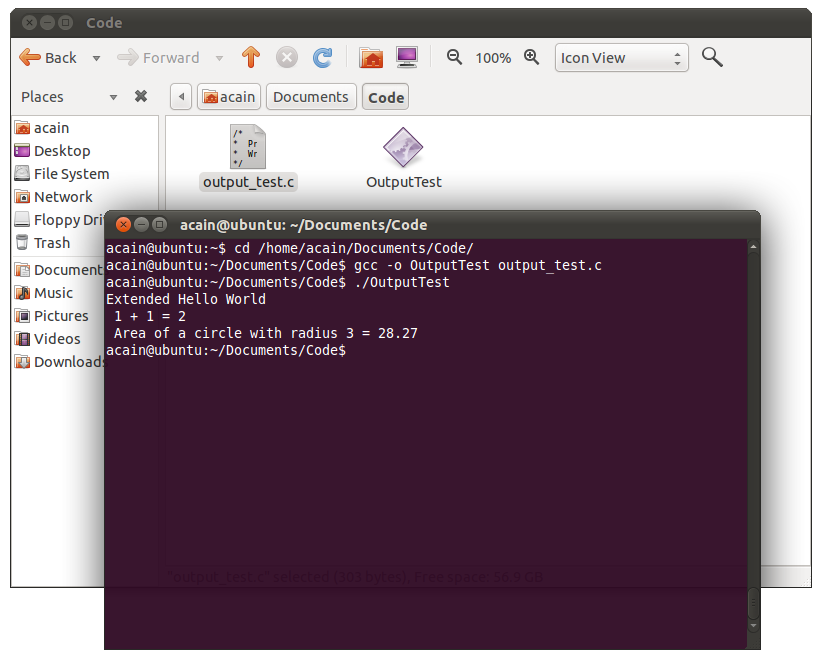
\includegraphics[width=0.62\textwidth]{./topics/program-creation/images/LinuxCompleteExample1} 
   \caption{Example of compiling and running a C version of Output Test on Linux}
   \label{fig:program-creation-complete-linux-version}
\end{figure}

\begin{figure}[h]
   \centering
   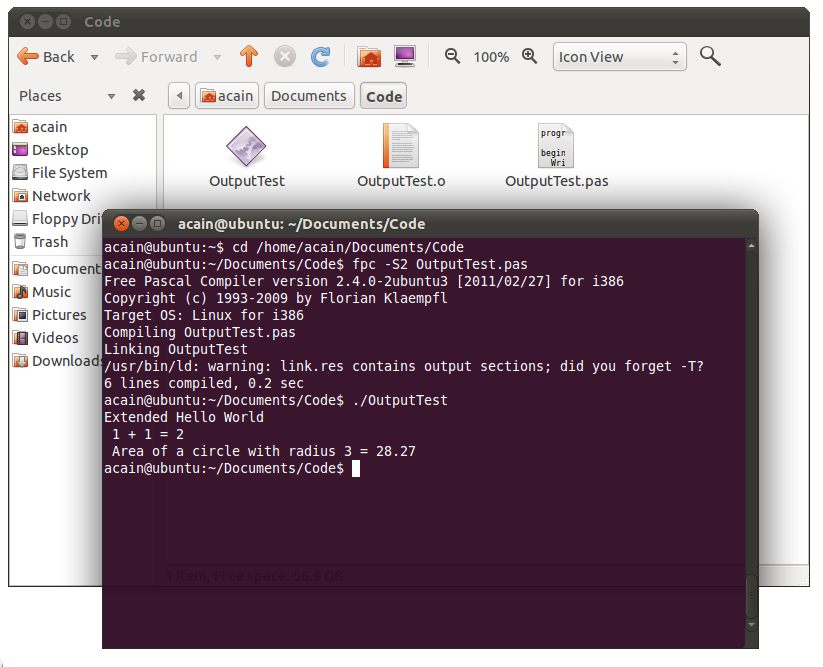
\includegraphics[width=0.62\textwidth]{./topics/program-creation/images/LinuxCompleteExample} 
   \caption{Example of compiling and running a Pascal version of Output Test on Linux}
   \label{fig:program-creation-complete-linux-version-1}
\end{figure}

\clearpage
Figure \ref{fig:program-creation-complete-macos-version} shows an example of the instructions needed to compile and run the C version of the \emph{Output Test} program on MacOS. Figure \ref{fig:program-creation-complete-macos-version-1} shows an example of the instructions needed to compile and run the Pascal version of the \emph{Output Test} program on MacOS.

\begin{figure}[h]
   \centering
   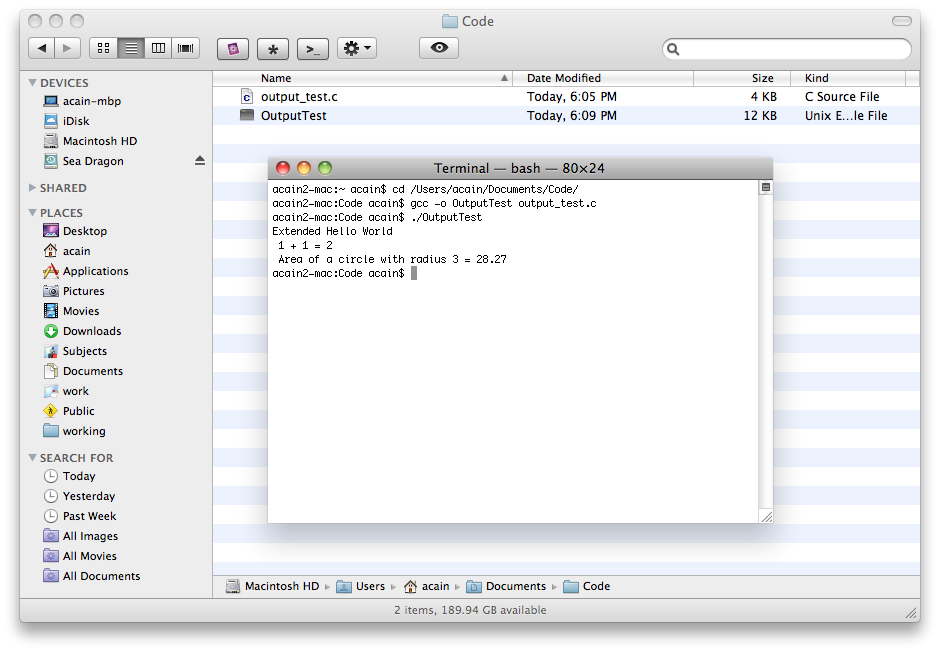
\includegraphics[width=0.73\textwidth]{./topics/program-creation/images/MacOSCompleteExample1} 
   \caption{Example of compiling and running a C version of Output Test on MacOS}
   \label{fig:program-creation-complete-macos-version}
\end{figure}

\begin{figure}[h]
   \centering
   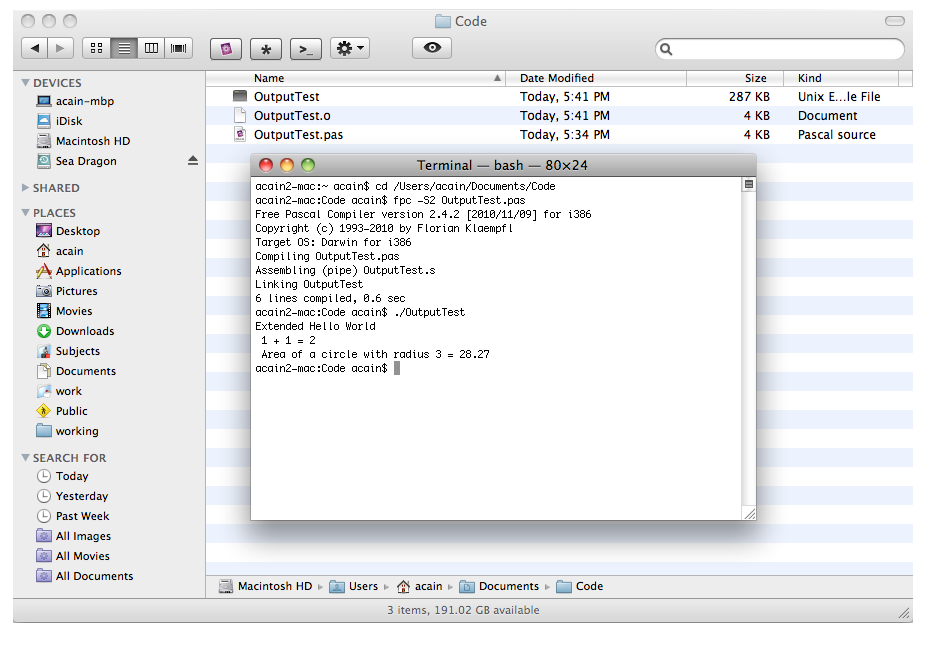
\includegraphics[width=0.73\textwidth]{./topics/program-creation/images/MacOSCompleteExample} 
   \caption{Example of compiling and running a Pascal version of Output Test on MacOS}
   \label{fig:program-creation-complete-macos-version-1}
\end{figure}

\clearpage
Figure \ref{fig:program-creation-complete-windows-version} shows an example of the instructions needed to compile and run the C version of the \emph{Output Test} program on MacOS. Figure \ref{fig:program-creation-complete-windows-version-1} shows an example of the instructions needed to compile and run the Pascal version of the \emph{Output Test} program on MacOS.

\begin{figure}[h]
   \centering
   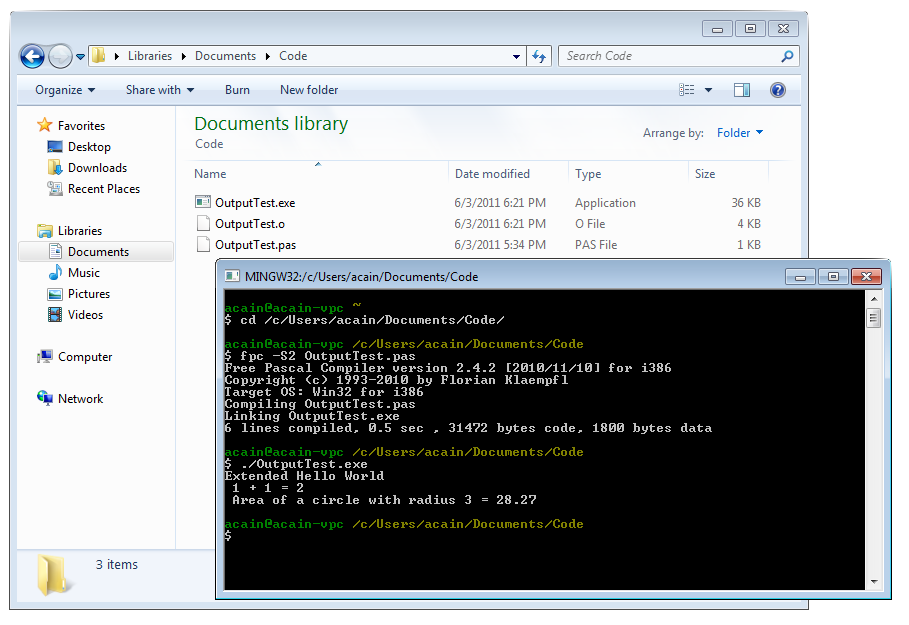
\includegraphics[width=0.73\textwidth]{./topics/program-creation/images/WindowsCompleteExample} 
   \caption{Example of compiling and running a C version of Output Test on Windows}
   \label{fig:program-creation-complete-windows-version}
\end{figure}

\begin{figure}[h]
   \centering
   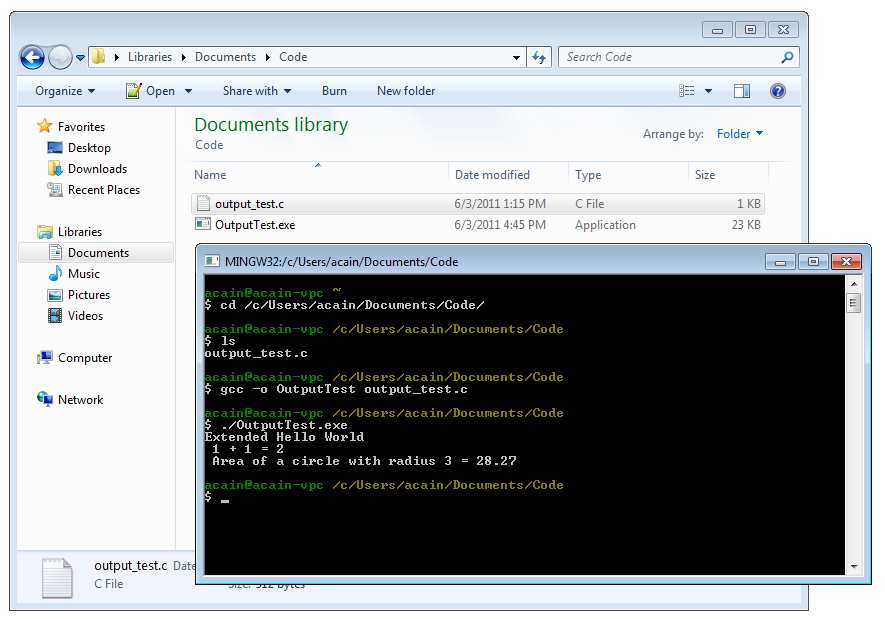
\includegraphics[width=0.73\textwidth]{./topics/program-creation/images/WindowsCompleteExample1} 
   \caption{Example of compiling and running a C version of Output Test on Windows}
   \label{fig:program-creation-complete-windows-version-1}
\end{figure}

% subsection compiling_and_running_output_test (end)
\clearpage
\subsubsection{Compiler Errors} % (fold)
\label{ssub:compiler_errors}

The compiler is a very sensitive piece of software. It requires that you follow the language's syntax precisely. One small mistake, and the compiler will fail to compile your program and end with an error message. This is further complicated by the fact that in many cases the compiler's error messages can appear cryptic.

Here are some handy hints related to dealing with compiler errors.

\begin{enumerate}
  \item \textbf{Know that errors are inevitable}. You will get compiler errors. As you gain more experience you will get fewer errors, but it will always be a rare event that everything is exactly as it should be the first time.
  \item \textbf{Start with the first error message, and do not move on until its fixed}. The compiler will read your code from the top down. So the first error it outputs will be the first in the file. The problem is that the compiler will try to continue on, despite the error. This can mean that other errors further on it the output were actually caused by the compiler being \emph{confused} due to the first error. By fixing the first error you may also fix subsequent errors, as you gain experience you will learn to work out which errors are genuine, and which were caused by previous errors.
  \item \textbf{Deal with one error at a time}. Its easy to feel overwhelmed when you see a huge list of errors, but do not be scared off. Start at the first error, and solve them one by one. Compile after fixing each problem to see if the others are real, or if they were a result of the previous error.
  \item \textbf{Do not add more code until the errors are fixed}. Compile your program frequently. Add small pieces of functionality, and then fix any syntax errors before adding the next piece of functionality. Coding in this way makes sure that you should not get too many errors, and reduces the code you have to search in order to fix the problem.
  \item \textbf{Read the error message carefully}. The message will try to tell you what has gone wrong, and once you understand what the messages are trying to say you will be able find and fix the issues quickly.
  \item  \textbf{Work out what the error messages mean}. Understanding the error messages will mean that you will know what to look for, and will help you avoid these errors in the future. If your not sure what an error message means ask others developers or search for the message on the internet.
  \item \textbf{Find the line and character number of the error}. One important detail in the error message will be the line number of the error. This gives you a starting point to help you locate the problem. Its important to note that this is where the compiler got to when it noticed the error. This \emph{does not} guarantee that this is where the error actually is, but it is a good place to start looking. In some cases this will be the location of the error, in others you may need to look back one or more lines to find the actual source of the problem.
  \item \textbf{Watch for typos}. It is easy to mistype an identifier. When this happens the compiler will not know what to do. Make sure you check for these tiny typos when you get errors related to the compiler not being able to find an identifier.
  \item \textbf{When you get stuck ask for help}. Compiler errors are likely to be something small, but something these small things are hard to find. If you get stuck ask for help. Having access to other more experienced developers will be a valuable resource as you learn to program. Learning to program can be tough at times, and having someone who can help you will make all the difference.
\end{enumerate}


% subsubsection compiler_errors (end)

